%%%%%%%%%%%%%%%%%%%%%%%%%%%%%%%%%%%%%%%%%%%%%%%%%%%%%%%%%%%%%%%%%%%%%%%%%%%%%%%
% Uni Duesseldorf
% Lehrstuhl fuer Datenbanken and Informationssysteme
% Vorlage fuer Bachelor-/Masterarbeiten
% Optimiert fuer den Original-Latex-Kompiler LATEX.EXE (LaTeX=>PS=>PDF)
% Version 1.4 - 2.3.2010
%%%%%%%%%%%%%%%%%%%%%%%%%%%%%%%%%%%%%%%%%%%%%%%%%%%%%%%%%%%%%%%%%%%%%%%%%%%%%%%

%%%%%%%%%%%%%%%%%%%%%%%%%%%%%%%%%%%%%%%%%%%%%%%%%%%%%%%%%%%%%%%%%%%%%%%%%%%%%%%
%%%%%%%%%%% BEGINN EINSTELLUNG FUER DIE ARBEIT. UNBEDINGT ERFORDERLICH! %%%%%%%
%%%%%%%%%%%%%%%%%%%%%%%%%%%%%%%%%%%%%%%%%%%%%%%%%%%%%%%%%%%%%%%%%%%%%%%%%%%%%%%
% Geben Sie Ihren Namen hier an
\newcommand{\bearbeiter}{Alina Elterman}

% Geben Sie hier den Titel Ihrer Arbeit an
\newcommand{\titel}{Game-theoretic Analysis of Strategyproofness in Cake-cutting Protocols}

% Geben Sie das Datum des Beginns and Ende der Bachelorarbeit ein
\newcommand{\beginndatum}{05. September 2011}
\newcommand{\abgabedatum}{05.~Dezember~2011}

% Geben Sie die Namen des Erst- and Zweitgutachters an
\newcommand{\erstgutachter}{Prof. Dr.~J\"org Rothe}
\newcommand{\zweitgutachter}{Prof. Dr.~Peter Kern}

% Falls Sie die Arbeit zweiseitig ausdrucken wollen,
% benutzen Sie die folgende Zeile mit
% \AN fuer zweiseitigen Druck
% \AUS fuer einseitigen Druck
\newcommand{\zweiseitig}{\AUS}

% Falls die Arbeit in englischer Sprache verfasst 
% werden soll, dann benutzen Sie die folgende Zeile mit
% englisch fuer englische Sprache
% deutsch fuer deutsche Sprache
\newcommand{\sprache}{englisch}
%%%%%%%%%%%%%%%%%%%%%%%%%%%%%%%%%%%%%%%%%%%%%%%%%%%%%%%%%%%%%%%%%%%%%%%%%%%%%%%%%
%%%%%%%%%%%%%%%%%%%%%%%%%%%%%%% ENDE EINSTELLUNGEN %%%%%%%%%%%%%%%%%%%%%%%%%%%%%%
%%%%%%%%%%%%%%%%%%%%%%%%%%%%%%%%%%%%%%%%%%%%%%%%%%%%%%%%%%%%%%%%%%%%%%%%%%%%%%%%%

% Die folgende Zeile NICHT EDITIEREN oder loeschen
% (Zum Ab�ndern der BA-Vorlage in eine MA-Vorlage muessen sie
% jedoch die Datei titelmakros1.tex selbst editieren.)
%%%%%%%%%%%%%%%%%%%%%%%%%%%%%%%%%%%%%%%%%%%%%%%%%%%%%%%%%%%
% Obere Titelmakros. Editieren Sie diese Datei nur, wenn
% Sie sich ABSOLUT sicher sind, was Sie da tun!!!
% (Z.B. zum Abaendern der BA-Vorlage in eine MA-Vorlage)
% Uni Duesseldorf
% Lehrstuhl fuer Datenbanken und Informationssysteme
% Version 2.2 - 2.3.2010
%%%%%%%%%%%%%%%%%%%%%%%%%%%%%%%%%%%%%%%%%%%%%%%%%%%%%%%%%%%
\newcommand{\AN}{twoside}
\newcommand{\AUS}{}
%\newcommand{\englisch}{}
%\newcommand{\deutsch}{\usepackage[german]{babel}}

%% Die folgenden auskommentierten Optionen dienen der automatischen
%% Erkennung des Latex-Kompilers und dem Setzen der davon abh�ngigen
%% Einstellungen. Bei Problem z.B. mit dem Einbinden von verschiedenen
%% Grafiktypen bei Verwendung von PdfLatex oder Latex, einfach die
%% verschiedenen \usepackage(s) ausprobieren. (Mit diesen Einstellungen
%% funktionierte diese Vorlage bei der Verwenundg von latex.exe als
%% Kompiler bei den meisten Studierenden.)

%\newif\ifpdf \ifx\pdfoutput\undefined
%\pdffalse % we are not running pdflatex
%\else
%\pdfoutput=1 % we are running pdflatex
%\pdfcompresslevel=9 % compression level for text and image;
%\pdftrue \fi

\documentclass[11pt,a4paper, \zweiseitig]{article}



%\usepackage[iso]{umlaute}
\usepackage[latin1]{inputenc}
\usepackage{palatino} % palatino Schriftart
%\usepackage{makeidx} % um ein Index zu erstellen
\usepackage{tocbibind}
\usepackage[T1]{fontenc} %fuer richtige Trennung bei Umlauten
\usepackage{fancybox} % fuer die Rahmen
\usepackage{shortvrb}
\usepackage{ifthen}
\ifthenelse{\equal{\sprache}{deutsch}}{\usepackage[ngerman]{babel}}{}

\usepackage{lmodern} 
\usepackage{amsmath}
\usepackage{amssymb}
\usepackage{pdfpages}
\usepackage{hyperref}
%\usepackage{fancyheadings}
\usepackage{fancyhdr}
\usepackage{amsfonts}
\usepackage{amsthm}
\usepackage{color}
\usepackage{stmaryrd}
\usepackage{nomencl}
\usepackage[normalem]{ulem} 
\newcommand{\markup}[1]{\uline{#1}}
% Befehl umbenennen in abk
\let\abk\nomenclature

\usepackage{a4wide} % ganze A4 Weite verwenden

%\ifpdf
%\usepackage[pdftex,xdvi]{graphicx}
%\usepackage{thumbpdf} %thumbs fuer Pdf
%\usepackage[pdfstartview=FitV]{hyperref} %anklickbares Inhaltsverzeichnis
%\else
\usepackage[dvips,xdvi]{graphicx}
\usepackage{hyperref} %anklickbares Inhaltsverzeichnis
%\fi

%%%%%%%%%%%%%%%%%%%%%%% Massangaben fuer die Arbeit %%%%%%%%%%%%%%%
\setlength{\textwidth}{15cm}

\setlength{\oddsidemargin}{35mm}
\setlength{\evensidemargin}{25mm}

\addtolength{\oddsidemargin}{-1in}
\addtolength{\evensidemargin}{-1in}

%\makeindex
% Umgebungen f"ur S�tze usw.
\newtheorem*{bemerkung*}{Bemerkung}
\newtheorem*{defi}{Definition}
\newtheorem*{defi*}{Definition}
\newtheorem*{bezeichnungen}{Bezeichnungen}
\newtheorem*{fakt}{Fakt}
\newtheorem*{beispiel}{Beispiel}
\newtheorem*{bsp}{Beispiel}
\newtheorem*{beispiel*}{Beispiel}
\newtheorem*{satz}{Satz}
\newtheorem*{satz*}{Satz}
\newtheorem*{lem}{Lemma}
\newtheorem*{protokoll*}{Protokoll}
\newtheorem*{idee}{Idee}

%definition of new commands
\newcommand{\DGEF}{\text{\textbf{DGEF}}}

\begin{document}

%\setcounter{secnumdepth}{4} %Nummerieren bis in die 4. Ebene
%\setcounter{tocdepth}{4} %Inhaltsverzeichnis bis zur 4. Ebene

\pagestyle{headings}

\sloppy % LaTeX ist dann nicht so streng mit der Silbentrennung
\MakeShortVerb{\�}

\parindent0mm
\parskip0.5em


{
\textwidth170mm 
\oddsidemargin30mm 
\evensidemargin30mm 
\addtolength{\oddsidemargin}{-1in}
\addtolength{\evensidemargin}{-1in}

\parskip0pt plus2pt

% Die Raender muessen eventuell fuer jeden Drucker individuell eingestellt
% werden. Dazu sind die Werte fuer die Abstaende `\oben' und `\links' zu
% aendern, die von mir auf jeweils 0mm eingestellt wurden.

%\newlength{\links} \setlength{\links}{10mm}  % hier abzuaendern
%\addtolength{\oddsidemargin}{\links}
%\addtolength{\evensidemargin}{\links}

\begin{titlepage}
\vspace*{-1.5cm}
  \raisebox{17mm}{
    \begin{minipage}[t]{70mm}
      \begin{center}
        %\selectlanguage{german}
        {\Large INSTITUT F�R INFORMATIK\\}
        {\normalsize
          Lehrstuhl f�r Komplexit\"atstheorie und Kryptologie
\\
        }
        \vspace{3mm}
        {\small Universit�tsstr. 1 \hspace{5ex} D--40225 D�sseldorf\\}
     \end{center}
    \end{minipage}
  }
  \hfill
  
\includegraphics[width=130pt]{bilder/HHU_Logo}
  \vspace{14em}

% Titel
  \begin{center}
      	\baselineskip=55pt
    	\textbf{\huge \titel}
  	 	\baselineskip=0 pt
   \end{center}

  %\vspace{7em}

\vfill

% Autor
  \begin{center}
    \textbf{\Large
      \bearbeiter
    }
  \end{center}

  \vspace{35mm}
 
% Pr�fungsordnungs-Angaben
  \begin{center}
    %\selectlanguage{german}
    
%%%%%%%%%%%%%%%%%%%%%%%%%%%%%%%%%%%%%%%%%%%%%%%%%%%%%%%%%%%%%%%%%%%%%%%%%
% Ja, richtig, hier kann die BA-Vorlage zur MA-Vorlage gemacht werden...
%%%%%%%%%%%%%%%%%%%%%%%%%%%%%%%%%%%%%%%%%%%%%%%%%%%%%%%%%%%%%%%%%%%%%%%%%
    {\Large Bachelorarbeit}

    \vspace{2em}

    \begin{tabular}[t]{ll}
      Beginn der Arbeit:& \beginndatum \\
      Abgabe der Arbeit:& \abgabedatum \\
      Gutachter:         & \erstgutachter \\
                         & \zweitgutachter \\
    \end{tabular}
  \end{center}

\end{titlepage}

}

%%%%%%%%%%%%%%%%%%%%%%%%%%%%%%%%%%%%%%%%%%%%%%%%%%%%%%%%%%%%%%%%%%%%%
\clearpage
\begin{titlepage}
  ~                % eine leere Seite hinter dem Deckblatt
\end{titlepage}
%%%%%%%%%%%%%%%%%%%%%%%%%%%%%%%%%%%%%%%%%%%%%%%%%%%%%%%%%%%%%%%%%%%%%
\clearpage
\begin{titlepage}
\vspace*{\fill}

\section*{Erkl�rung}

%%%%%%%%%%%%%%%%%%%%%%%%%%%%%%%%%%%%%%%%%%%%%%%%%%%%%%%%%%%
% Und hier ebenfalls ggf. BA durch MA ersetzen...
%%%%%%%%%%%%%%%%%%%%%%%%%%%%%%%%%%%%%%%%%%%%%%%%%%%%%%%%%%%

Hiermit versichere ich, dass ich diese Bachelorarbeit
selbstst�ndig verfasst habe. Ich habe dazu keine anderen als die
angegebenen Quellen und Hilfsmittel verwendet.

\vspace{25 mm}

\begin{tabular}{lc}
D�sseldorf, den \abgabedatum \hspace*{2cm} & \underline{\hspace{6cm}}\\
& \bearbeiter
\end{tabular}

\vspace*{\fill}
\end{titlepage}

%%%%%%%%%%%%%%%%%%%%%%%%%%%%%%%%%%%%%%%%%%%%%%%%%%%%%%%%%%%%%%%%%%%%%
% Leerseite bei zweiseitigem Druck
%%%%%%%%%%%%%%%%%%%%%%%%%%%%%%%%%%%%%%%%%%%%%%%%%%%%%%%%%%%%%%%%%%%%%

\ifthenelse{\equal{\zweiseitig}{twoside}}{\clearpage\begin{titlepage}
~\end{titlepage}}{}

%%%%%%%%%%%%%%%%%%%%%%%%%%%%%%%%%%%%%%%%%%%%%%%%%%%%%%%%%%%%%%%%%%%%%
\clearpage
\begin{titlepage}

\section*{\ifthenelse{\equal{\sprache}{deutsch}}{Zusammenfassung}{Abstract}}


%%%%%%%%%%%%%%%%%%%%%%%%%%%%%%%%%%%%%%%%%%%%%%%%%%%%%%%%%%%%%%%%%%%%%%%%%%%%%%%%%
%%%%%%%%%%%%%%%%%%%%%%%%%%%% BEGINN ZUSAMMENFASSUNG %%%%%%%%%%%%%%%%%%%%%%%%%%%%%
%%%%%%%%%%%%%%%%%%%%%%%%%%%%%%%%%%%%%%%%%%%%%%%%%%%%%%%%%%%%%%%%%%%%%%%%%%%%%%%%%
\begin{enumerate}
\item What is the problem?
\item Why interesting?
\item How to solve?
\item What is the result?
\end{enumerate}

%%%%%%%%%%%%%%%%%%%%%%%%%%%%%%%%%%%%%%%%%%%%%%%%%%%%%%%%%%%%%%%%%%%%%%%%%%%%%%%%%
%%%%%%%%%%%%%%%%%%%%%%%%%%%%% ENDE ZUSAMMENFASSUNG %%%%%%%%%%%%%%%%%%%%%%%%%%%%%%
%%%%%%%%%%%%%%%%%%%%%%%%%%%%%%%%%%%%%%%%%%%%%%%%%%%%%%%%%%%%%%%%%%%%%%%%%%%%%%%%%

% Die folgende Zeile NICHT EDITIEREN oder loeschen
%%%%%%%%%%%%%%%%%%%%%%%%%%%%%%%%%%%%%%%%%%%%%%%%
% Untere Titelmakros. Editieren Sie diese Datei nur, wenn Sie sich
% ABSOLUT sicher sind, was Sie da tun!!!
%%%%%%%%%%%%%%%%%%%%%%%%%%%%%%%%%%%%%%%%%%%%%%%
\vspace*{\fill}
\end{titlepage}

%%%%%%%%%%%%%%%%%%%%%%%%%%%%%%%%%%%%%%%%%%%%%%%%%%%%%%%%%%%%%%%%%%%%%
% Leerseite bei zweiseitigem Druck
%%%%%%%%%%%%%%%%%%%%%%%%%%%%%%%%%%%%%%%%%%%%%%%%%%%%%%%%%%%%%%%%%%%%%
\ifthenelse{\equal{\zweiseitig}{twoside}}
  {\clearpage\begin{titlepage}~\end{titlepage}}{}
%%%%%%%%%%%%%%%%%%%%%%%%%%%%%%%%%%%%%%%%%%%%%%%%%%%%%%%%%%%%%%%%%%%%%
\clearpage 
\tableofcontents
\thispagestyle{empty}
%\enlargethispage{\baselineskip}
\clearpage \setcounter{page}{1}
%%%%%%%%%%%%%%%%%%%%%%%%%%%%%%%%%%%%%%%%%%%%%%%%%%%%%%%%%%%%%%%%%%%%%
% Leere Seite, falls Inhaltsverzeichnis mit ungerader Seitenzahl und 
% doppelseitiger Druck
%%%%%%%%%%%%%%%%%%%%%%%%%%%%%%%%%%%%%%%%%%%%%%%%%%%%%%%%%%%%%%%%%%%%%
\ifthenelse{ \( \equal{\zweiseitig}{twoside} \and \not \isodd{\value{page}} \)}
	{\pagebreak \thispagestyle{empty} \cleardoublepage}{\clearpage}



%%%%%%%%%%%%%%%%%%%%%%%%%%%%%%%%%%%%%%%%%%%%%%%%%%%%%%%%%%%%%%%%%%%%%
%%%%%%%%%%%%%%%%%%%%%%%%% BEGINN TEXTTEIL %%%%%%%%%%%%%%%%%%%%%%%%%%%
%%%%%%%%%%%%%%%%%%%%%%%%%%%%%%%%%%%%%%%%%%%%%%%%%%%%%%%%%%%%%%%%%%%%%
\section{Introduction}
Cake cutting is an interdisciplinary field which is commonly researched and part of economics, political science, mathematics, operations research, and computer science. Game theory is fulfilling the same property. Except for this fact, they have hardly something in common. While cake cutting is about fair division of a heterogeneous divisible good, game theory studies the strategies people use when making decisions.\\
The role of strategies have not been widely researched yet in the context of cake cutting. But their importance is indisputable. Just imagine the following situation:
\\
\newline
%Example Cost Sharing from Algorithmic GT Noam Nissan chap. 15
%\begin{itemize}
%\item{division of sports tickets, health resources, computer networking resources, voting power, intellectual property licenses, costs for environmental improvements, etc}
%\item{formalize fairness, including max-min fairness, proportional fairness, envy-free fairness, etc. which may or may not lead to stable allocations in the sense of say Nash Equilibrium, or strong Nash Equilibrium}
%\end{itemize}
\pagebreak

\section{Preliminaries}
\subsection{Preliminaries of Game Theory}
GT is about ... 
Game theory consist of two fields: cooperative and non-cooperative.\\ The first one is about single selfish player, and in the second one the main focus is on forming coalitions. For compter scientist especially the algorithmic game theory is of major interest. 
\begin{defi}{\textbf{(Game)}}
A 
\end{defi}
\begin{defi}{\textbf{(Pay-off)}}
A Egalitarian and utiletarian
\end{defi}

\begin{bsp}
\label{bsp2}
(Cooperative Cake-Cutting)\\
After the win of the election in Turingville the member of President Church coalition want to divide succesfully the power in the country. 
\end{bsp}
\newpage
\subsection{Preliminaries of Cake-cutting}
\subsubsection{Basics}
Before starting, it is necessary to define the components of cake-cutting. Example \ref{bsp1} sketches the problem statement.\\
%
\begin{bsp}
\label{bsp1}
Cook, Younger and Kasami got a cheese-chocolate-straberry-cake. 
\end{bsp}
%
Now, what exactly is cake-cutting about? First of all, it involves a discrete set of $n \in \mathbb{N}$ agents (or players ) $P_n=\{p_1,\cdots,p_n\}$. It is assumed that each of them want to get as much as possible of the divided good. The goal is to allocate it in a manner that the players are satisfied. Hereby only the value of their own piece imply the degree of satisfiabily of the players. The allocation of a single, divisible and heterogeneous good is included in the consideration of this work.\\ 
	\begin{figure}[h]
		\centering
 		 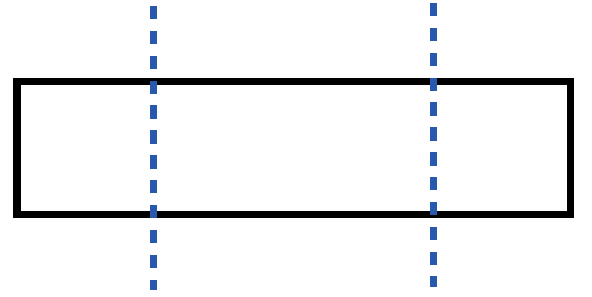
\includegraphics[width=130pt]{kek.pdf}
   \caption{Cake}[Example for a visualisation of a cake and two cuts]
  	 \end{figure}
It is common to use for the visualization a rectangular cake. The division is performed by parallel cuts.\\ The cake $X$ is represented by the unit interval $I=[0,1] \subseteq \mathbb{R}$. Each subinterval $I'\subseteq I$ or a union of subintervals $\sideset{}{ }\bigcup\limits_{m\in\mathbb{N}}I_m$ 
with $I_m\subseteq I$ is called a bundle (piece), which are disjoint. The bundle of the cake, which the player $p_i$ receives is denoted as $X_i$. When all bundles of the cake are owned by players, this state is called an \underline{allocation}. Each piece has a public length, which can be computed as the sum of all border differences, and the private value of each player.\\

Every player $p_i\in P_n$ has a \underline{valuation function (valuation)} $v_i:\{X'|X' \subseteq X\} \mapsto [0,1]$ on the cake $X$ with the following properties:
\begin{enumerate}
\item Non-negativity: $v_i(C)\geq 0$ for all $C\subseteq [0,1].$
\item Normalisation: $v_i(\emptyset)=0$ and $v_i([0,1])=1.$
\item Additivity: $v_i(C \cup C')=v_i(C)+v_i(C')$ for disjoint
$C,C'\subseteq [0,1].$\footnote{Monotonicity: If $C' \subseteq C$ then $v_i(C') \leq v_i(C)$ follows from additivity, because for the assumption $C' \subseteq C$ and $A:=C\backslash C'$: $v_i(C)=v_i(A\cup C')=v_i(A)+v_i(C')=\underbrace{v_i(C\backslash C')}_{\geq 0}+v_i(C')\geq v_i(C')$}
\item Divisibility: For all $C\subseteq [0,1]$ and all $\alpha \in
\mathbb{R}$, $0\leq \alpha \leq 1$, exist a $B\subseteq C$, so that
$v_i(B)=\alpha \cdot v_i(C).$
\item  $v_i$ is continuous: If $0<x<y\leq 1$ with $v_i([0,x])=\alpha$ and
$v_i([0,y])=\beta$, than for every $\gamma \in [\alpha,\beta]$ there exist a $z \in [x,y]$ so that $v_i([0,z])=\gamma.$
\item Emptyness of single points:  $v_i([x,x])=0$ for all $x\in [0,1].$
\end{enumerate}

\textbf{Different Types of Fairness}\\
\newline
Especially the fairness plays an important role in fair division. But what is fair? It can be seen as an valuation criteria of an allocation, which can be normalized and gives a possibility to compare different allocations. Usually the fairness criteria are distinguished between the following:\\
\begin{defi}{\textbf{(Proportional or simple fair)}}
\newline An allocation is \underline{proportional (simple fair)}, if
$v_i(X_i) \geq 1/n$ for each player $p_i \in P_N$.
\end{defi}
\begin{defi}{\textbf{(Envy-freeness)}}
\newline An allocation is \underline{envy-free}, if $v_i(X_i) \geq
v_i(X_j)$ for each couple of players $p_i, p_j \in P_N$.
\end{defi}
\begin{defi}{\textbf{(Equity)}}
\newline An allocation is \underline{equitable}, if $v_i(X_i) =
\alpha$ for each player $p_i \in P_N$ and $0 \leq \alpha \leq 1$ \footnote{ If $\alpha = 1/n$ the allocation is called \underline{exact}.}.
\end{defi}
%
\textbf{Correlation between the Fairness-Properties}
\begin{lem}
For all allocations:
\begin{enumerate}
\item Every envy-free allocation is proportional.
\item For two players an allocation is envy-free iff it is proportional.
\end{enumerate}
\end{lem}
\begin{proof}
\begin{enumerate}
\item Every envy-free allocation is proportional.
\item For two players an allocation is envy-free iff it is proportional.
\end{enumerate}
\end{proof}
A slighly different criteria to valuate the performance of an allocation is the efficiency. The correlation between the fairness criterion and efficiency can be found in \cite{chen:truth} and \cite{brams}. 
\begin{defi}{\textbf{(Efficiency)}}
\newline An allocation $A=\{A_1,\dots, A_n\}$ is \underline{efficient (Pareto optimal)} if there is no other allocation $A'=\{A'_1,\dots, A'_n\}$ such that $v_i(A_i)\leq v_i(A'_i)$ for all players $p_i \in P_n$ and for at least one player the inequality is strict.
\end{defi}
\begin{lem}
For all allocations:
	\begin{enumerate}
		\item Envy-freeness does not imply efficiency.
		\item Pareto optimality does not ensure fairness
	\end{enumerate}
\end{lem}

\begin{proof}
	\begin{enumerate}
		\item Envy-freeness does not imply efficiency.
		\item Allocating all the cake to one player is Pareto optimal, but definitely not proportional and so not envy-free.
	\end{enumerate}
\end{proof}
\newpage

\subsubsection{Strategyproofness}
In the wide spectrum of literature diffent definitions and specifications about the honesty of players occur. Since the origin is game-theoretic and the main research is done in mechanism design, which is a part of game theory, the start will be there. In practise players are usually selfish, and try to increase the value of their bundle. In order to do so, they may report false valuations on parts of the cake. The goal is to prevent those happening.
\begin{defi}{\textbf{(Risk Aversion)}}
A player is \underline{risk averse} if .
\end{defi}

\begin{defi}{\textbf{(Strategyproofness)}}
\end{defi}

\begin{defi}{\textbf{(Truthfully)}}
An allocation is \underline{truthful} if the value of the cake obtained by a player by reporting false is not greater than by reporting the truth.
\end{defi}


\begin{defi}{\textbf{(Truthfully in expectation)}}
An allocation is \underline{truthful in expectation} if there .
\end{defi}

Only such divisions are interesting, in which each player acts truthfully by following his best strategy $\Sigma_{i}$.
%
It is common that if a player deviates from $\Sigma_{i}$ he risks to loose the guaranty for his fair share. At the end of an allocation it can be proven whether every player got his fair share. 
Each protocol 

\newpage
\textbf{Different Types of Protocols}\\
\newline
Due to the fact that the protocols are going to be analysed in this work, it is very important to understand the types, structure and design of them.\\
\newline
\textbf{Classes of Protocols}\\
\newline
Informal: (Algorithm)
\newline In mathematics, computer science and related subjects, an
\underline{algorithm} is an effective method for solving a problem, which can be denoted as a finite set of sequences.
\begin{defi}{\textbf{(Protocol (Cake-Cutting-Protocol))}}
\newline A \underline{protocol (cake-cutting-protocol)} is an adaptive algorithm with a fixed number of players and the following properties:
\begin{itemize}
\item{It consists of rules and strategies.\\ \underline{Rules} are requirements, which has to be followed by the players without knowledge of their valuations.\\
\underline{Strategies} are recommendations, which can be followed for getting the guaranteed fair share.}
\item{If a player does not follow the strategy of a protocol, he looses his guarantee to get a fair piece of cake after a fixed number of steps. His actions does not harm the other players.}
\item Each player should be able to cut the cake at a required moment independent of other players.
\item The protocol has no information about the valuation of the players, except of those, it got from the steps before. And so cannot prove whether a player follows the strategy of the protocol.
\end{itemize}
\end{defi}
\begin{bsp}
Cut and Choose\\
\begin{tabular*}{\textwidth}[]{|ccc|}
\hline
\hline
&\textbf{Cut $\&$ Choose for $n=2$}&\\
\end{tabular*}
\begin{tabular*}{\textwidth}[]{|l|c|r|}
\hline
\textbf{Rules}& \textbf{Player $p_1$ strategy}& \textbf{Player $p_2$ strategy}\\
\hline
1. Player $p_1$ partition &Partition $X$ into two&\\
the cake $X$ into two&pieces of equal size&\\
pieces $\{X',X-X'\}$&&\\
\hline
2. Player $p_2$ chooses&&Choose the bigger piece\\
one piece&&\\
\hline
3. Player $p_1$ get the &&\\remaining piece&&\\
\hline
\end{tabular*}
\end{bsp}
\begin{satz}
Cut $\&$ choose is strategyproof.
\end{satz}
\begin{proof}
\textbf{Options for not following the recomended strategy:}
\begin{itemize}
\item Player $p_2$ take the smaller piece. This can not be in his intention, because then he is less satiesfied after the basic assumption.
\item Player $p_1$ cut the cake into two not equal pieces. The chance to get less is equal to the chance to get more of the cake. In stochastic terms it means, that the expected value at the end of the allocation will be in the honest case: $ \frac{1}{2} \cdot \frac{1}{2}+\frac{1}{2} \cdot \frac{1}{2}=\frac{1}{2} $ and in the dishonest case: $ \frac{1}{2} \cdot X' +\frac{1}{2} \cdot (X-X') =\frac{1}{2} \cdot \underbrace{X}_{=1}=\frac{1}{2}$. It is defined, that in the case with equal outcomes the player would stay honest.
\end{itemize}
\end{proof}

\begin{defi}
A cake-cutting protocol is called \underline{proportional} or \underline{envy-free}, if independent of the valuation of the players, each allocation is proportional or envy-free under the requirement, that all players follows the rules and strategies given by the protocol.
\end{defi}
The development of such protocols is one of the main goals of cake-cutting.

\begin{defi}{\textbf{(finite (discrete)/ continuous)}}
\newline A \underline{finite (discrete)} protocol gives a solution after a finite number of queries (valuations, marks, $\ldots$), in comparison in a \underline{continuous} protocol has a player to make infinitely many queries.
\end{defi}
\begin{defi}{\textbf{(finite bounded/ finite unbounded))}}
\newline A \underline{finite bounded} protocol has an upper bound of steps for all possible valuations. The number of those steps is only correlated, in some cases, with the number of players. A \underline{finite unbounded} protocol has no approximated number of steps.
\end{defi}
\begin{defi}{\textbf{(Moving Knife))}}
\newline A \underline{moving knife} protocol ...
\end{defi}
The most desirable protocols are the finite bounded, because they are the easiest to realise in real life applications. 
\pagebreak
\subsection{The Degree of Guaranteed Envy-Freeness}
In the last sixty years the number of proportional finite bounded protocols have grown for arbitrary n.\\But still no envy-free finite bounded protocol for an arbitrary $n$ exist. The biggest group we can divide a cake in a fixed number of steps, so that it is envy-free, is sadly three.\\ As a compromise between envy-freeness and finite boundness and a possibility to value proportional cake-cutting protocols between each other is the degree of guaranteed envy-freeness from \cite{lindner:degrees}. 

\begin{defi}
 For an allocation of the cake $X=\bigcup\limits_{i=1}^n X_i$ for the players $P=\{p_1,\dots,p_n\}$:
 \begin{itemize}
  \item An \underline{envy relation} $\Vdash$ is a binary relation on $P$ %$(\Vdash, PxP)$
  $:p_i$ envies 
        $p_j$ $(p_i\Vdash p_j)$, $1\leq i,j\leq n,$ $i\neq j$, if $v_i(X_i)<v_i(X_j)$.
  \item An \underline{envy-free relation} $\nVdash$ is a binary relation on $P:p_i$ not envies $p_j$ $(p_j
        \nVdash p_j)$ ,$1\leq i,j\leq n$ ,$i\neq j$, if $v_i(X_i)\geq v_i(X_j)$.
 \end{itemize}
\end{defi}
\underline{Properties of $\Vdash$ and $\nVdash$:}
\begin{itemize}
 \item $\Vdash$ is irreflexive.
 \item $\nVdash$ is reflexive.
 \item $\Vdash$ and $\nVdash$ are not transitive
 \end{itemize}
\begin{proof}
	\begin{itemize}
 		\item $v_i(X_i)<v_i(X_i)$ is never possible.
 		\item $v_i(X_i)\geq v_i(X_i)$ is always satisfied, but the trivial relation $p_i \nVdash p_i$ does not count.
 		\item Let $p_i\Vdash p_j$ and $p_j\Vdash p_k$, but about $v_i(X_k)$ nothing can be concluded: $p_i\nVdash p_k$ is still possible
	\end{itemize}
\end{proof}
$\Rightarrow$ No proposition can be concluded about symmetry. So the following is possible:
\begin{enumerate}
 \item Two-Way-Envy: $p_i\Vdash p_j$ and $p_j\Vdash p_i$\\(Exchange of the portions makes both happy.)
 \item Two-Way-Envyfreeness: $p_i\nVdash p_j$ and $p_j\nVdash p_i$\\(No exchange necessary.)
 \item One-Way-Envy: $p_i\Vdash p_j$ and $p_j\nVdash p_i$\\
       One-Way-Envyfreeness: $p_j\Vdash p_i$ and $p_i\nVdash p_j$
\end{enumerate}
%\begin{beispiel*}
 %Aufteilung $X=X_F\cup X_G\cup X_H$ des Kuchens mit\\
 %\begin{tabular}{c|ccc}
  %& $X_F=$\begin{tabular}{ccc}&&$\Box$\\&$\Box$&$\Box$\\$\Box$&$\Box$&$\Box$\\1&2&3\end{tabular}
  %& $X_G=$\begin{tabular}{ccc}$\Box$&$\Box$&$\Box$\\7&8&9\end{tabular}
  %& $X_H=$\begin{tabular}{ccc}$\Box$&$\Box$&$\Box$\\$\Box$&$\Box$&$\Box$\\4&5&6\end{tabular}\\ \hline \\
  %F & \textcolor{blue}{$\frac{6}{18}=\frac{1}{3}$} & $\frac{6}{18}=\frac{1}{3}$ & $\frac{6}{18}=\frac{1}{3}$\\ \\
  %G & $\frac{9}{18}=\frac{1}{2}$ & \textcolor{blue}{$\frac{3}{18}=\frac{1}{6}$} & $\frac{6}{18}=\frac{1}{3}$\\ \\
  %H & $\frac{5}{18}$ & $\frac{7}{18}$ & \textcolor{blue}{$\frac{6}{18}=\frac{1}{3}$}
 %\end{tabular}\\
 %$\Rightarrow$ nicht proportional wegen $v_G(X_g)=\frac{1}{6}<\frac{1}{3}$.\\
 %Es gibt:
 %\begin{itemize}
 % \item[] Ein-Weg-Neid von $G$ zu $F$:\\$G\Vdash F$ wegen $v_G(X_G)=\frac{1}{6}<v_G(X_F)=\frac{1}{2}$
  %        \\ Gleichzeitig ist dies\\$F\nVdash G$ wegen $v_F(X_G)=\frac{1}{3}=v_F(X_F)$
  %\item[] Ein-Weg-Neidfreiheit von $F$ zu $G$
  %\item[] Zwei-Wege-Neidfreiheit zwischen $F$ and $H$\\ $F\nVdash H$, da $v_F(X_F)=\frac{1}{3}=v_F(X_H)$\\
   %       $H\nVdash F$, da $v_H(X_H=\frac{6}{18}>\frac{5}{18}=v_H(X_F)$
  %\item[] Zwei-Wege-Neid zwischen $G$ and $H$\\$G\Vdash H$, da $v_g(X_G)=\frac{1}{6}<\frac{1}{3}=v_G(X_H)$\\
   %       $H\Vdash G$, da $v_H(X_H)=\frac{1}{3}<\frac{7}{18}=v_H(X_G)$
 %\end{itemize}
 %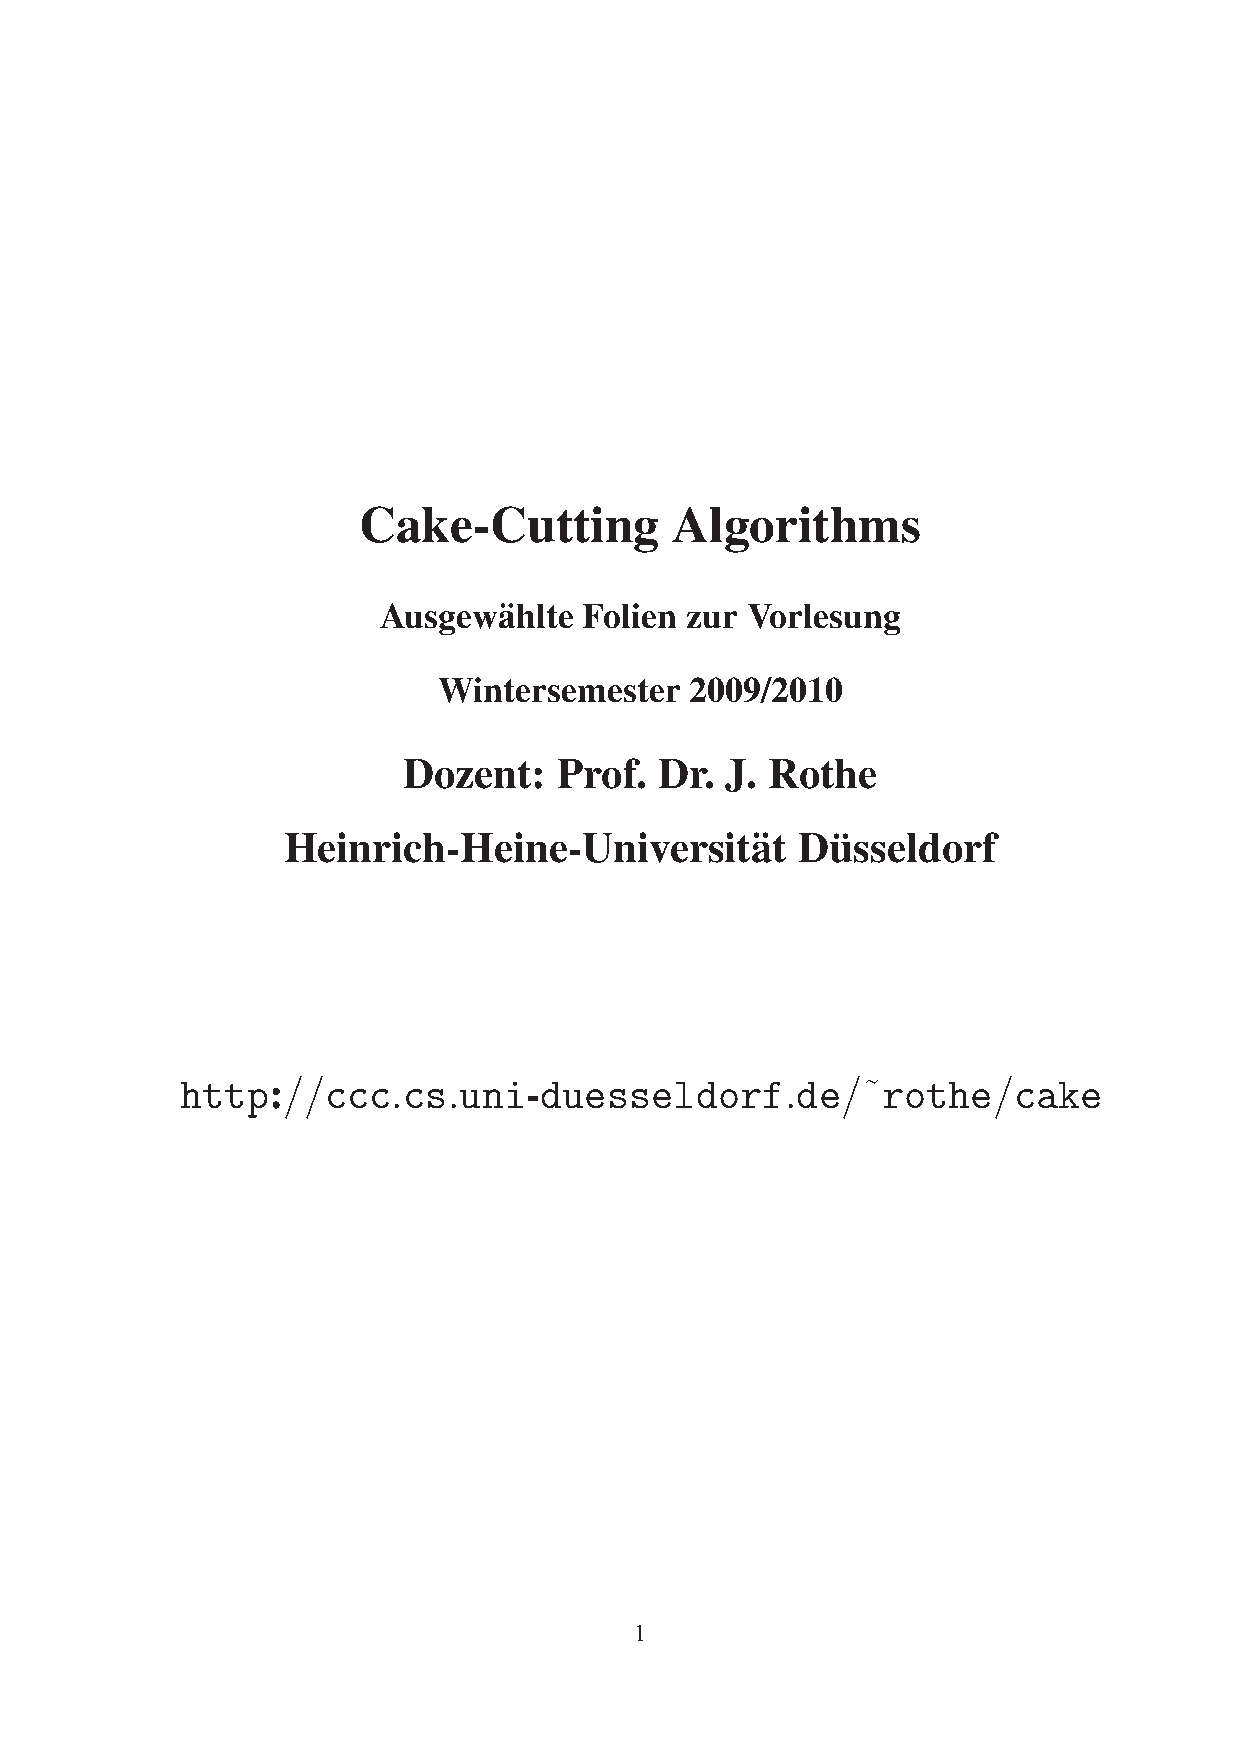
\includepdf[pages=KästchenfolieBis9,scale=0.8]{folien.pdf}
%\end{beispiel*}
\underline{$\DGEF$} = Smallest number of envy-free-relations for all possible valuations.
\begin{protokoll*}
 Chomsky and Turing use cut $\&$ choose at a conference with $n$ other scientists.\\
 $\DGEF: 2(n-1)+(n-2)(n-2)=2n-2+n^2-4n+4=n^2-2n+2$
\end{protokoll*}
\begin{satz*}
 \begin{enumerate}
  \item Each envy-free cake-cutting protocol with $n\geq1$ players has a $\DGEF = n(n-1)$.
  \item Let $d(n)$ be the notation for the $\DGEF$ of a proportional cake-cutting protocols with $n\geq2$ players. Then: $n\leq d(n)\leq n(n-1)$.
 \end{enumerate}
\end{satz*}
NEU MACHEN!!!
\begin{proof}
 \begin{enumerate}
  \item $p_i\nVdash p_i$ for all $i$, $1\leq i\leq n$, can be ignored, so has each of the $n$ player to each other player, an envy-free-relation, summarized to $n(n-1)$.
  \item \begin{description}
         \item[$n=2$] Obviosly: $d(2)=2$, because the cake-cutting protocol is proportional: $v_1(X_1)\geq\frac{1}{2}$ and $v_2(X_2)\geq\frac{1}{2}
                    \Rightarrow v_1(X_1)\geq v_1(X_2)$ and $v_2(X_2)\geq v_2(X_1)$
         \item[$n\geq3$] Because $p_i\nVdash p_i$ for all $i$ are ignored, $d(n)\leq n(n-1)$.
                         \begin{itemize}
                          \item[] In a proportional allocation:\\$v_i(X_i)\geq\frac{1}{n}$ for $1\leq i\leq n$.\\
                          \item[$\Rightarrow$] None of the $n$ players can simultaneously envy all other players, because:\\
                                               In the contrary assumption: $p_1\nVdash p_2$
                          \item[$\Rightarrow$]$v_1(X_2)>v_1(X_1)\geq\frac{1}{n}$
                          \item[$\Rightarrow$]$v_1((X-X_1)-X_2)<\frac{n-2}{n}$
                          \item[$\Rightarrow$]$(X-X_1)-X_2$ cannot be allocated in $n-2$ portions, so that $v_i(X_j)\geq\frac{1}{n}$
                                              for all $j,3\leq j\leq n$.
                          \item[$\Rightarrow$] it exists a $j,3\leq j\leq n$, so that $v_i(X_j)<\frac{1}{n}$.
                          \item[$\Rightarrow$]$p_i\nVdash p_j$
                         \end{itemize}
                         So has each of the $n$ players at least one guaranteed envy-free-relation to an other player: $n\leq d(n)$  
        \end{description}
 \end{enumerate}
\end{proof}
STOP!
\begin{satz}
 If the rules/strategies of a proportional cake-cutting protocols with $n\geq2$ player never require from a player to value the portion of an other player the $\DGEF=n$.
\end{satz}
\begin{proof}
 \begin{description}
  \item[$n=2$] Proportionality $\Rightarrow$ Envy-freeness\\$\DGEF=2 \cdot 1=n(n-1)$
  \item[$n\geq3$] Imagine the following case: For a given allocation $X=\bigcup\limits_{i=1}^nX_i$, which is proportional, but require no other limitations, lets assume the following valuations: \\For each $i, 1\leq i\leq n$, value of $p_i$:
                  \begin{itemize}
                   \item the own piece $X_i$ with $v_i(X_i)=\frac{1}{n}=\frac{n}{n^2}\Rightarrow$ proportional!
                   \item the piece $X_j$ of a player $p_j, j\neq i: v_i(X_j)=\frac{2}{n}<\frac{1}{n}$
                   \item each of the $n-2$ other pieces $X_k$ of the players $p_k, |{i,j,k}|=3, v_i=(X_k)=\frac{n+1}{n^2}>\frac{1}{n}$
                  \end{itemize}
                  In summary for each $i, 1\leq i\leq n$:
                  \begin{enumerate}
                   \item $v_i(X)=v_i(\bigcup\limits_{j=1}^nX_j)\stackrel{\text{Additivity}}{=}\sum\limits_{j=1}^nv_i(X_j)=
                         \frac{1}{n^2}(n+2+(n-2)(n+1))=\frac{1}{n^2}(n+2+n^2+n-2n-2)=1$
                   \item $p_i$ has $n-2$ envy-relations and only one envy-free-relation\\$\Rightarrow$ There are $n$ guaranteed envy-free-relations, each for every player.
                  \end{enumerate}
 \end{description}
\end{proof}
\textbf{Overview: DGEF of proportional cake-cutting protocols}\\
\begin{tabular*}{\textwidth}{@{\extracolsep{\fill}}|l|l|l|}
\hline
Protocol & DGEF & $n=4$ (12 EF)  \\
\hline
Last Diminisher & $2+\frac{n\cdot(n-1)}{2}$&8\\
\hline
Lone Chooser & $n$&4\\
\hline
Lone Divider & $2n-2$&6\\
\hline
Cut your Own Piece & $n$&4\\
\hline
Cut your Own Piece (left-right rule) & $2n-2$&6\\
\hline
Divide $\&$ Conquer & $n\cdot \lfloor log (n)\rfloor +2n-2^{\lfloor log (n)\rfloor +1}$&6\\
\hline
Minimal-Envy Divide $\&$ Conquer & $n\cdot \lfloor log (n)\rfloor +2n-2^{\lfloor log (n)\rfloor +1}$&6\\
\hline
Recursive Divide $\&$ Choose & $n$&4\\
\hline
Parallel Last Diminisher & $\lceil \frac{n^2}{2} \rceil + 1$&9\\
\hline
\end{tabular*}

\begin{corollary}
The performance of the protocols have the following order for $n\geq 2$:\\
$n \leq 2n-2 \leq n\cdot \lfloor log (n)\rfloor +2n-2^{\lfloor log (n)\rfloor +1} \leq 2 + \frac{n(n-1)}{2} \leq \lceil \frac{n^2}{2} \rceil + 1$
\end{corollary}

\begin{proof}
$n=2$: $2 \leq 2 \leq 2 \leq 3 \leq 3$\\
$n \mapsto n+1$ \\$n+1 \leq 2n \rightarrow 2n-n-1=n-1 \geq 0$\\
$2n \leq n\cdot \lfloor log (n+1)\rfloor +2n+2-2^{\lfloor log (n+1)\rfloor +1} \rightarrow n\cdot \lfloor log (n+1)\rfloor +2n+2-2^{\lfloor log (n+1)\rfloor +1}-2n=n\cdot \lfloor log (n+1)\rfloor-2^{\lfloor log (n+1)\rfloor} \geq 0$
\end{proof}
\pagebreak

\section{Proportional Protocols and their DGEF}
Each proportional protocol consists of rules and strategies. Since the rules are compulsory, it is optional for the player to follow the strategies.\\
In this chapter the strategies of common used procedures are described. First of all, the protocols are rewritten into a game-theoretic manner. Then their strategyproofness is analysed. During complications the effect on the DGEF is shown. Complete protocols in the standart describtion can be found in \cite{robertson:cake-cutting}.
\subsection{The Steinhaus-Kuhn Lone Divider Procedure}

\newpage
\subsection{The Banach-Knaster Last-Diminisher Procedure}
The generalization of ''I cut, you choose''.
\begin{satz}
If the valuations of the players are not equal, there exist a non truthful strategy for the first player in each round of getting a piece with $v_i(S_i)>1/N$.\\
\end{satz}
\begin{proof}
The player $p_1$ got the piece $X_1$. So $v_1(X_1)=1/n$ and for all $p_i$ with $2\leq i\leq n$ $v_i(X_1)<1/n$. W.l.o.g. in the assumption, let $\delta=1/n-v_2(X_1)$. It is obvious that $\delta > 0$.\\
Step 1: The piece which was cutted schould have the value $1/N+\epsilon$  with $\epsilon =$ residue of $S_1$.\\
Destinction of cases: Either player $p_1$ get this piece or player $p_i$ cut it and so player $p_1$ can get a piece with same properties in the next roundor during Cut and Choose in the end.
\end{proof}
\begin{satz}
 The Last-Diminisher-protocol has a $\DGEF$ of $\frac{n(n-1)}{2}+2$.
\end{satz}
%\begin{proof}
 %\begin{description}
  %\item[Runde 1] Sei $\bar{p}_1$ der Spieler, der die erste Portion erhalt. %Jeder andere Spieler bewertet diese mit $\leq\frac{1}{n}$,
%                 beneidet also $\bar{p}_1$ nicht\\$\Rightarrow n-1$ garantierte Neidfrei-Relationen
%  \item[Runde $i, 1<i<n$] Analog zu Runde 1 konnen $n-i$ Neidfrei-Relationen garantiert werden. $\bar{p}_i$, der die ite Portion erhalt, wird
%                          von den verbleibenden Spielern nicht beneidet.\\$\Rightarrow$ mindestens $\sum\limits_{i=1}^ni=\frac{n-1}{2}$
%                          garantierte Neidfrei-Relationen
%  \item[Letzte Runde] \begin{enumerate}
%                       \item Cut \& Choose zwischen $\bar{p}_{n-1}$ and $\bar{p}_n$. Keiner dieser beiden beneidet den anderen.\\
%                             $\Rightarrow$ eine zusatzliche garantierte Neidfrei-Relation.
%                       \item Da Last-Diminisher proportional ist, gibt es eine weitere garantierte Neidfrei-Relation für $\bar{p}_1$
 %                     \end{enumerate}
% \end{description}
%$\Rightarrow\DGEF=\frac{(n-1)n}{2}+2$ 
%\end{proof}
\newpage
\subsection{The Fink Lone-Chooser Procedure}
\begin{satz}
 The Lone-Chooser procedure has a $\DGEF = n$.
\end{satz}
\begin{proof}
 No player value a foreign piece $\stackrel{\text{Theorem}}{\Longrightarrow}\DGEF=n$
\end{proof}
For the description of this protocol between two groups of players will be separated. Players in the first group $P_I={p_1, \dots, p_i}$ in the $i-1$ round have already their proportional piece. Assume that player $p_1$ owns the whole cake before the first round. The performance in each round is the following:\\
\newline
\begin{tabular*}{\textwidth}[]{|c|}
\hline
\hline
\textbf{The Fink Lone-Chooser Procedure for arbitrary $n$}\\
\end{tabular*}
\begin{tabular*}{\textwidth}[]{|l|c|r|}
\hline
\textbf{Rules}& \textbf{Players in $P_I$ strategy}& \textbf{Player $p_{i+1}$ strategy}\\
\hline
1. Players $P_I$ partition &Partition $X_i$ into $i+1$&\\
their piece $X_i$ into $i+1$&pieces of equal size&\\
pieces $\{X_{i,1},\dots, X_{i,i+1}\}$&&\\
\hline
2. Player $p_{i+1}$ chooses&&Choose the biggest piece of each \\
one piece of each player&&player\\
\hline
\end{tabular*}
\begin{satz}
Fink Lone-Chooser Procedure is strategyproof.
\end{satz}
\begin{proof}
\textbf{Options for not following the recomended strategy:}
\begin{itemize}
\item Player $p_{i+1}$ take the smaller piece. This can not be in his intention, because then he is less satiesfied after the basic assumption.
\item Players in $P_I$ cut the cake into $i+1$ not equal pieces. The chance that player $p_{i+1}$ take a certain piece is $\frac{1}{i+1}$. In stochastic terms it means, that the expected value at the end of the allocation will be in the honest case at least: $ i \cdot \frac{1}{i+1} \cdot \frac{1}{i} =\frac{1}{i+1} $ (because he had at least $\frac{1}{i}$ before) and in the dishonest case:\\
Assume the value of the piece will be distributed on $s$ pieces with $1 \leq s \leq i+1$. Then $ \frac{1}{i} \cdot \frac{i+1-s}{i+1} + \frac{s-1}{si}\cdot \frac{s}{i+1} =\frac{1}{i+1} $. Even if the value will be distributed inequally on the $s$ pieces, it would not affect the outcome, because the probability of the piece the player $p_{i+1}$ take is uniformly distributed.\\
 \newline It is defined, that in the case with equal outcomes the player would stay honest.
\end{itemize}
\end{proof}
\newpage
\subsection{The Cut-Your-Own-Piece Procedure}
\newpage
\subsection{The Divide-and-Conquer Procedure}
\newpage
\subsection{The Extended Procedure}
\newpage
\subsection{The Extension of the Extended Procedure}
\newpage
\section{Related Work}


\pagebreak

\section{Conclusions and Open Questions/Problems}
To take a closer look on the DGEF in the egalitarien point of view. Since a protocol is only fair if every player get his fair share, it seems to be intuitive more fair, if $n-1$ player envies one rather than one player envies all other. The definition could be:\\
MDGEF= minimal guaranteed degree of envy-freeness = $\min\limits_{i\in \mathbb{N}}\{\sum\limits_{j\in\mathbb{N},i \neq j} p_i \nVdash p_j\}$
 
\pagebreak

%%%%%%%%%%%%%%%%%%%%%%%%%%%%%%%%%%%%%%%%%%%%%%%%%%%%%%%%%%%%%%%%%%%%%%%%%%
%%%%%%%%%%%%%%%%%%%%%%%%%%%%%%% ENDE TEXTTEIL %%%%%%%%%%%%%%%%%%%%%%%%%%%%
%%%%%%%%%%%%%%%%%%%%%%%%%%%%%%%%%%%%%%%%%%%%%%%%%%%%%%%%%%%%%%%%%%%%%%%%%%

\clearpage
\bibliography{references.bib}
\bibliographystyle{alphadin}

%\vspace*{\fill}

\clearpage

\listoffigures

\listoftables

%\pagebreak

%\printindex
\end{document}